\documentclass[letterpaper]{article}


%%% Macros
%%% ------------------------------------------------------------
\newlength{\spacebox}
\settowidth{\spacebox}{8888888888}			% Box to align text
\newcommand{\sepspace}{\vspace*{1em}}		% Vertical space macro

\newcommand{\MyName}[1]{ % Name
		\Huge \usefont{OT1}{phv}{b}{n} \hfill #1
		\par \normalsize \normalfont}
		
\newcommand{\MySlogan}[1]{ % Slogan (optional)
		\large \usefont{OT1}{phv}{m}{n}\hfill \textit{#1}
		\par \normalsize \normalfont}

\newcommand{\NewPart}[1]{\section*{\uppercase{#1}}}

\newcommand{\PersonalEntry}[2]{
		\noindent\hangindent=2em\hangafter=0 % Indentation
		\parbox{\spacebox}{        % Box to align text
		\textit{#1}}		       % Entry name (birth, address, etc.)
		\hspace{1.5em} #2 \par}    % Entry value

\newcommand{\SkillsEntry}[2]{      % Same as \PersonalEntry
		\noindent\hangindent=2em\hangafter=0 % Indentation
		\parbox{\spacebox}{        % Box to align text
		\textit{#1}}			   % Entry name (birth, address, etc.)
		\hspace{1.5em} #2 \par}    % Entry value	
		
\newcommand{\EducationEntry}[4]{
		\noindent \textbf{#1} \hfill      % Study
		\colorbox{Black}{%
			\parbox{6em}{%
			\hfill\color{White}#2}} \par  % Duration
		\noindent \textit{#3} \par        % School
		\noindent\hangindent=2em\hangafter=0 \small #4 % Description
		\normalsize \par}

\newcommand{\WorkEntry}[4]{				  % Same as \EducationEntry
		\noindent \textbf{#1} \hfill      % Jobname
		\colorbox{Black}{\color{White}#2} \par  % Duration
		\noindent \textit{#3} \par              % Company
		\noindent\hangindent=2em\hangafter=0 \small #4 % Description
		\normalsize \par}




%%% Custom sectioning (sectsty package)
%%% ------------------------------------------------------------
\usepackage{xcolor,sectsty,regexpatch}

\makeatletter

%% Modify the look of the section rule
\newcommand{\setsectionrulecolor}[1]{\colorlet{awesome-red}{#1}}
\setsectionrulecolor{black}% default
\xpatchcmd*{\SS@normsectionrule}% <cmd>
  {\rule}% <search>
  {\color{awesome-red}\rule}% <replace>
  {}{}% <success><failure>
\makeatother

%% Implement the section rule
\sectionfont{%			            % Change font of \section command
	%\usefont{OT1}{phv}{b}{n}%		% bch-b-n: CharterBT-Bold font
	\sectionrule{0pt}{0pt}{-5pt}{0.2pt}}                                  



\usepackage{hyperref}
\usepackage{geometry}
\usepackage{pdfpages}  % Permite adjuntar pdfs al final del documento
\usepackage{graphicx}%<----remove demo in your file
\usepackage{wrapfig}
\usepackage{lscape}
\usepackage{rotating}
\usepackage{epstopdf}
\usepackage{textcomp} % hace falta para poner apostrofe
%\usepackage[table]{xcolor} % para las tablas bonitas coloreadas. loads also »colortbl«
\usepackage{array} % necesario para formatear del tiron una columna de una tabla
\usepackage{booktabs}
%\usepackage{pbox} % necesario para introducir salto de linea en celdas de una tabla
\usepackage{longtable}
\usepackage{pdflscape}
\usepackage{lscape}
\usepackage{amsmath}
\newcommand\T{\textrm{T}}  % "true"
\newcommand\F{\textrm{F}}  % "false"



\pagenumbering{gobble}

% Uncomment the following lines to use the Palatino font.  Remove the
% [osf] bit if you don't like the old style figures.
%
\usepackage[T1]{fontenc}
\usepackage[osf]{mathpazo}
\usepackage{xcolor}
\definecolor{StrongRed}{RGB}{139,0,0}
\definecolor{DarkRed}{RGB}{200,0,0}
\definecolor{awesome-red}{HTML}{DC3522}
\definecolor{awesome-skyblue}{HTML}{0395DE}
\definecolor{gray}{HTML}{5D5D5D}
\definecolor{lightgray}{HTML}{999999}




% Set your name here
\def\name{\textcolor{StrongRed}{Antonio Ortega Jim\'enez}}

% The following metadata will show up in the PDF properties
\hypersetup{
  colorlinks = true,
  urlcolor = black,
  pdfauthor = {\name},
  pdfkeywords = { },
  pdftitle = {\name:  },
  pdfsubject = { },
  pdfpagemode = UseNone
}

\geometry{textheight=8.5in, textwidth=6in}

% Customize page headers
\pagestyle{myheadings}
\markright{\name}
\thispagestyle{empty}

% Customize section headings
% \usepackage{sectsty}
% \subsectionfont{\rmfamily\mdseries\itshape\large}

% Don't indent paragraphs.
\setlength\parindent{0em}

% Make lists without bullets
\renewenvironment{itemize}{
  \begin{list}{}{
    \setlength{\leftmargin}{1em}
  }
}{
  \end{list}
}

\begin{document}


\thispagestyle{empty}

\centerline{\LARGE\bf \name}

\vspace{0.1in}
\centerline{\textcolor{awesome-red}{\textsc{Computational Biochemist}}}


\vspace{0.25in}


\begin{minipage}[t]{0.6\textwidth}
  \textbf{Citizenship}: Spanish \\
  \textbf{Cell phone}: +34 664 661 687 \\
  \textbf{Email}: \href{mailto:antortjim@alum.us.es}{antortjim@alum.us.es} \\
  \textbf{Website}: \href{http://www.antortega.com}{antortega.com} \\
  
\end{minipage}
\begin{minipage}[t]{0.3\textwidth}
  \textbf{LinkedIn}: \href{http://www.linkedin.com/in/antortjim}{linkedin.com/in/antortjim} \\
   \textbf{SO careers}:\\
   \href{http://careers.stackoverflow.com/antortjim}{careers.stackoverflow.com/antortjim} \\

\end{minipage}

\section*{Awards}

\begin{itemize}

\item \textbf{2012 Best Huelva province high-school record} \\ Government of Andalusia \\ The two best high school students from the province of Huelva were awarded this prize.

\item \textbf{2008 Paco Anillo Award on Mathematics representing Huelva} \\ Andalusian Association for Mathematical Education THALES \\  A prize bestowed in every andalusian province upon the most genuine solution proposed to one of the exercises posed at the Mathematical contest undergone in the same year.
\end{itemize}


\section*{Computational skills}

\vspace{-2\baselineskip}
\renewcommand{\arraystretch}{1.5}
\begin{table}[!h]

\begin{centering}
\begin{longtable}{>{\bfseries}r p{4.5in}}

Data analysis & Coexpression networks, Phylogeny, High-throughput omics data (RNA-seq, ChIP-seq, microarrays, Variant Call) \\

Databases & NCBI, Ensembl, Pfam, Uniprot, Biomodels, GOrilla, KEGG \\

Software & Linux, Cytoscape, GATK, Tuxedo protocol, Trinity, CellDesigner, BLAST, IGV, HOMER, MACS \\

Text editor & Vim \\

R \& Bioconductor & ggplot2, GenomicFeatures, BSgenome, dplyr, phangorn, cummeRbund, edgeR, ChIPseeker, GenomicRanges, seqinr, limma, igraph \\

Other languages & Octave/MATLAB, Bash, LaTeX, Python, HTML, CSS  \\

\end{longtable}
\end{centering}
\end{table}

\renewcommand{\arraystretch}{1}



\section*{Education}


\begin{itemize}

  \item \textbf{2016-2018 University of Copenhagen}, Denmark \\ MSc in Bioinformatics \\ Prospective student
  

  \item \textbf{2012-2016 University of Seville}, Spain \\ BSc in Biochemistry, Biotechnology track \\
    \textbf{GPA}: 2.57/4.0. \textbf{Average}: 8.52/10 \\
  %\footnote{Computed as $1 + \frac{\mbox{10 based score} - 5}{5} \times 3 $}\\
  Honors on Statistics, Biosynthesis of Macromolecules, Human Genetics, and Bioinformatics
  
  \item \textbf{July 2015 Complutense University of Madrid}, Spain \\ Summer School on Bioinformatics \\ Mark achieved: 9/10
  
  \item \textbf{June 2012 Alto Conquero High School}, Huelva, Spain \\
  High School diploma on Health Sciences \\
  Mark achieved: 9.1 \\

\end{itemize}


\section*{Self Education}

\begin{itemize}

  \item \textbf{2015 Codecademy} \\ 
  Python Syntax Course
  
  \item \textbf{2016 University of Stanford} at Coursera \\
  Machine Learning with Andrew Ng
  
    
    
\end{itemize}

\section*{Portfolio}

\begin{itemize}

\item A listing of relevant projects in Bioinformatics carried out during my Bachelor of Science can be retrieved at \href{antortega.com/?p=bioinformatics-portfolio}{antortega.com/?p=bioinformatics-portfolio}.

\end{itemize}




\section*{\textit{Wet lab} experience}


\begin{itemize}

\item \textbf{2014 - 2015 Intern Student}, CIC Cartuja, Seville. \\
Collaborated with Drs. Muro and Vioque's group on the characterization of the \textit{sigE} gene promoter in \textit{Nostoc PCC7120}.

\item \textbf{2015 - 2016 Assistant Research Fellow}, CIC Cartuja, Seville. \\
Carried out my bachelor thesis on the heterologous expression of All1873, a hypothetical protein of unknown function from \textit{Nostoc PCC7120}, in \textit{E. coli}.

\end{itemize}



\section*{Languages}

\renewcommand{\arraystretch}{1.5}

\vspace{-0.5cm}

\begin{table}[!h]

\begin{centering}
\begin{longtable}{>{\bfseries}l l p{4.5in}}

Spanish & Native & \\

English & Full professional proficiency (CAE C1 Level)\\

French & Limited working competences (DELF B1) \\

\end{longtable}
\end{centering}
\end{table}

\renewcommand{\arraystretch}{1}

\section*{Volunteering}

\renewcommand{\arraystretch}{1.5}
\vspace{-1.5\baselineskip}
\begin{table}[!h]

\begin{centering}
\begin{longtable}{>{\bfseries}l p{4in}}

Sal\'on del Estudiante 2016 & High-school students were encouraged to study the Life Sciences through simple experimental performances. \\
\end{longtable}
\end{centering}
\end{table}
\renewcommand{\arraystretch}{1}


\section*{Hobbies}
%\vspace{-0.6cm}
%\textcolor{awesome-red}{\rule{432pt}{0.2pt}}
\begin{itemize}
\vspace{0.1cm}
\item I enjoy practising sports, particularly jogging and basketball, and I always try to move around Seville by bike. I really enjoy listening to rock and electronic bands like AC/DC and Prodigy. I am fond of learning languages and new cultures. What I love the most is hanging out with my friends and visiting the center of Seville, an astonishingly beautiful city. 

I was a boy scout until age 11.


\end{itemize}

\section*{Attitudes}
%\vspace{-0.6cm}
%\textcolor{awesome-red}{\rule{432pt}{0.2pt}} \vspace{-0.0cm}

\begin{itemize}
\item Self-learner, hard worker, restless, ambitious  and determined to master my bioinformatics skills.
\end{itemize}

\section*{Appendix}
%\vspace{-0.6cm}
%\textcolor{awesome-red}{\rule{432pt}{0.2pt}} \vspace{-0.0cm}
\begin{enumerate}

%\item \hyperlink{motivation}{Motivation letter} (English)

\item \hyperlink{premio_extraordinario}{Best Huelva province record diploma} (Spanish)
\item \hyperlink{complu}{Summer School on Bioinformatics at Complutense University} (Spanish)
\item \hyperlink{exp-en}{Official college transcript of results} (English)
\item \hyperlink{cae}{Certificate in Advanced English} (English)
\end{enumerate}
%
%\clearpage

% Motivation letter

%\hypertarget{motivation}{}
%\includepdf[pages={1,2}]{carta/Antonio_Ortega_Motivation_Letter.pdf}
%\clearpage

% Diploma del premio extraordinario

\thispagestyle{empty}
\newgeometry{margin=20pt, bottom=5pt}
\hypertarget{premio_extraordinario}{}
\begin{landscape}
\centering
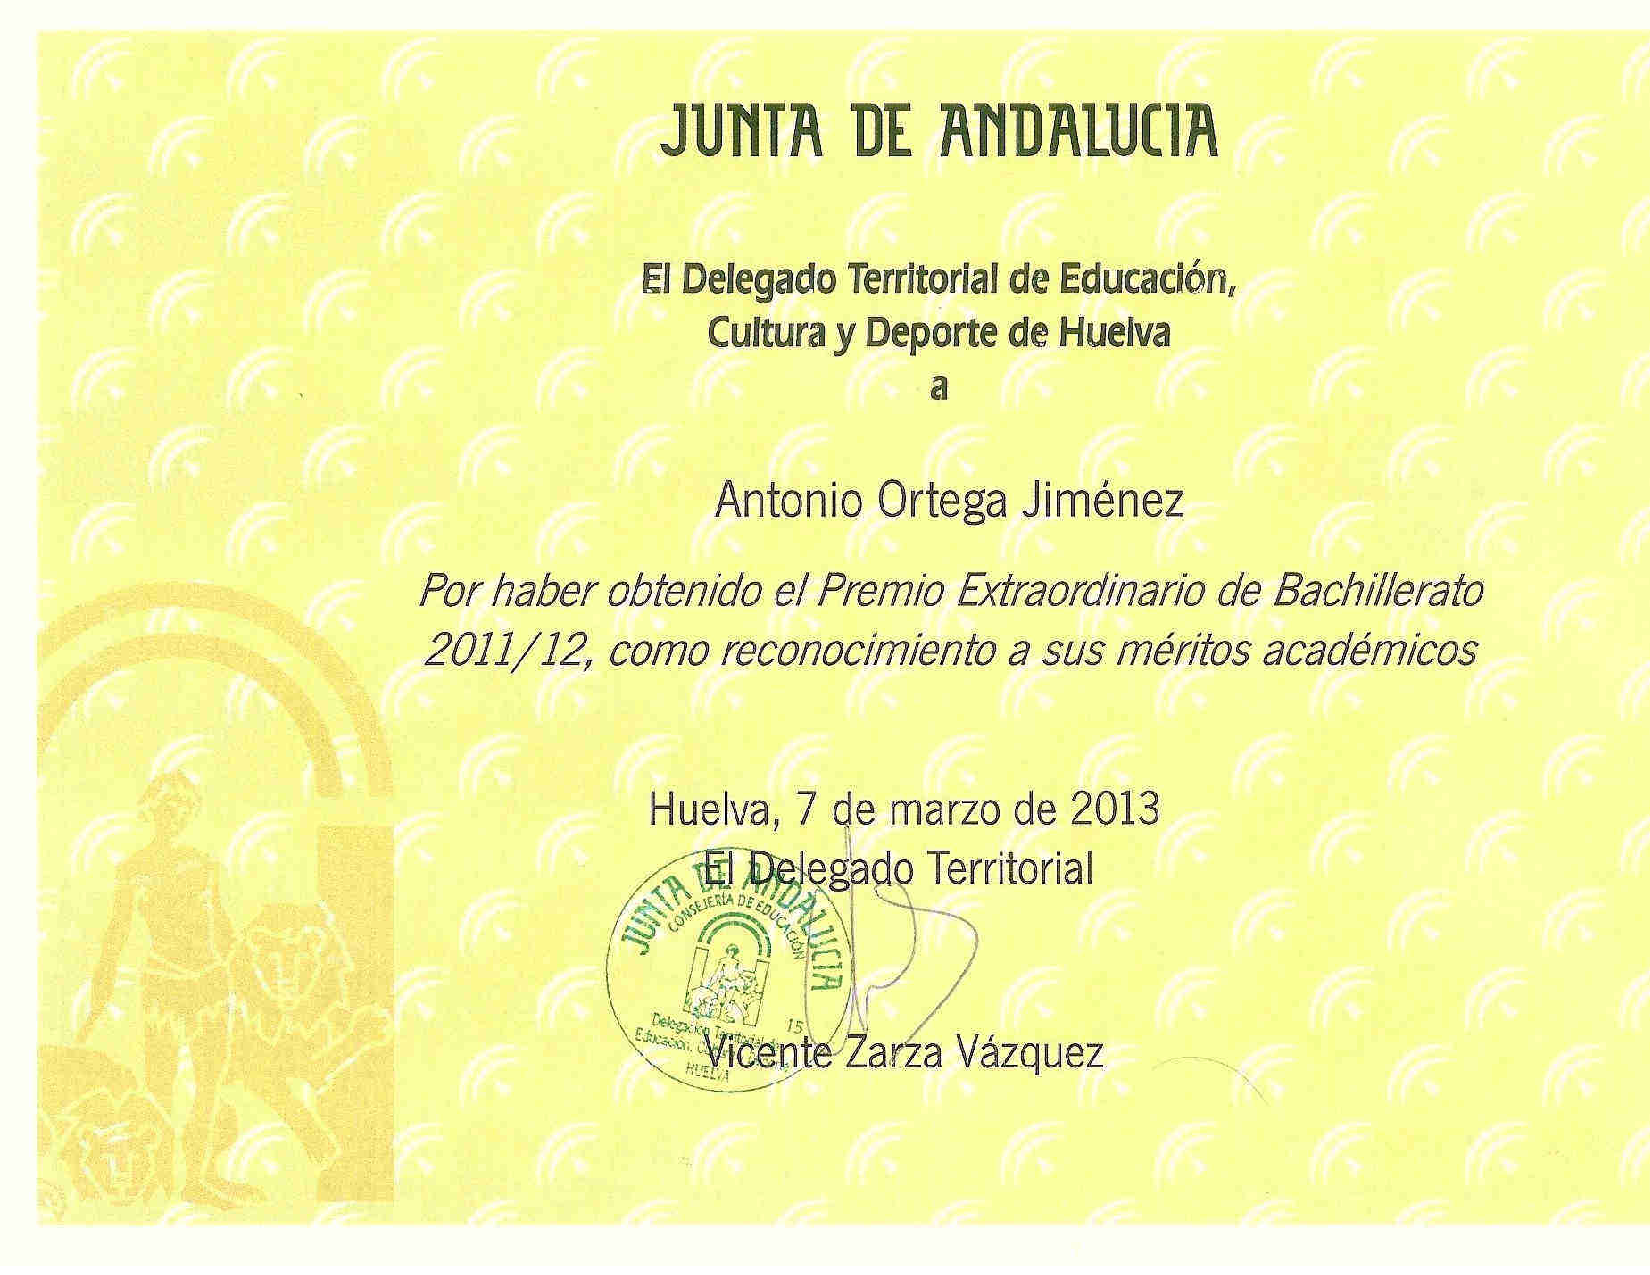
\includegraphics[scale=0.9]{./premio_extraordinario.pdf}
\end{landscape}
\restoregeometry
\clearpage


% Diploma del curso de bioinformatica en la complu
\thispagestyle{empty}

\newgeometry{margin=20pt, bottom=5pt}
\hypertarget{complu}{}
\begin{landscape}
\centering
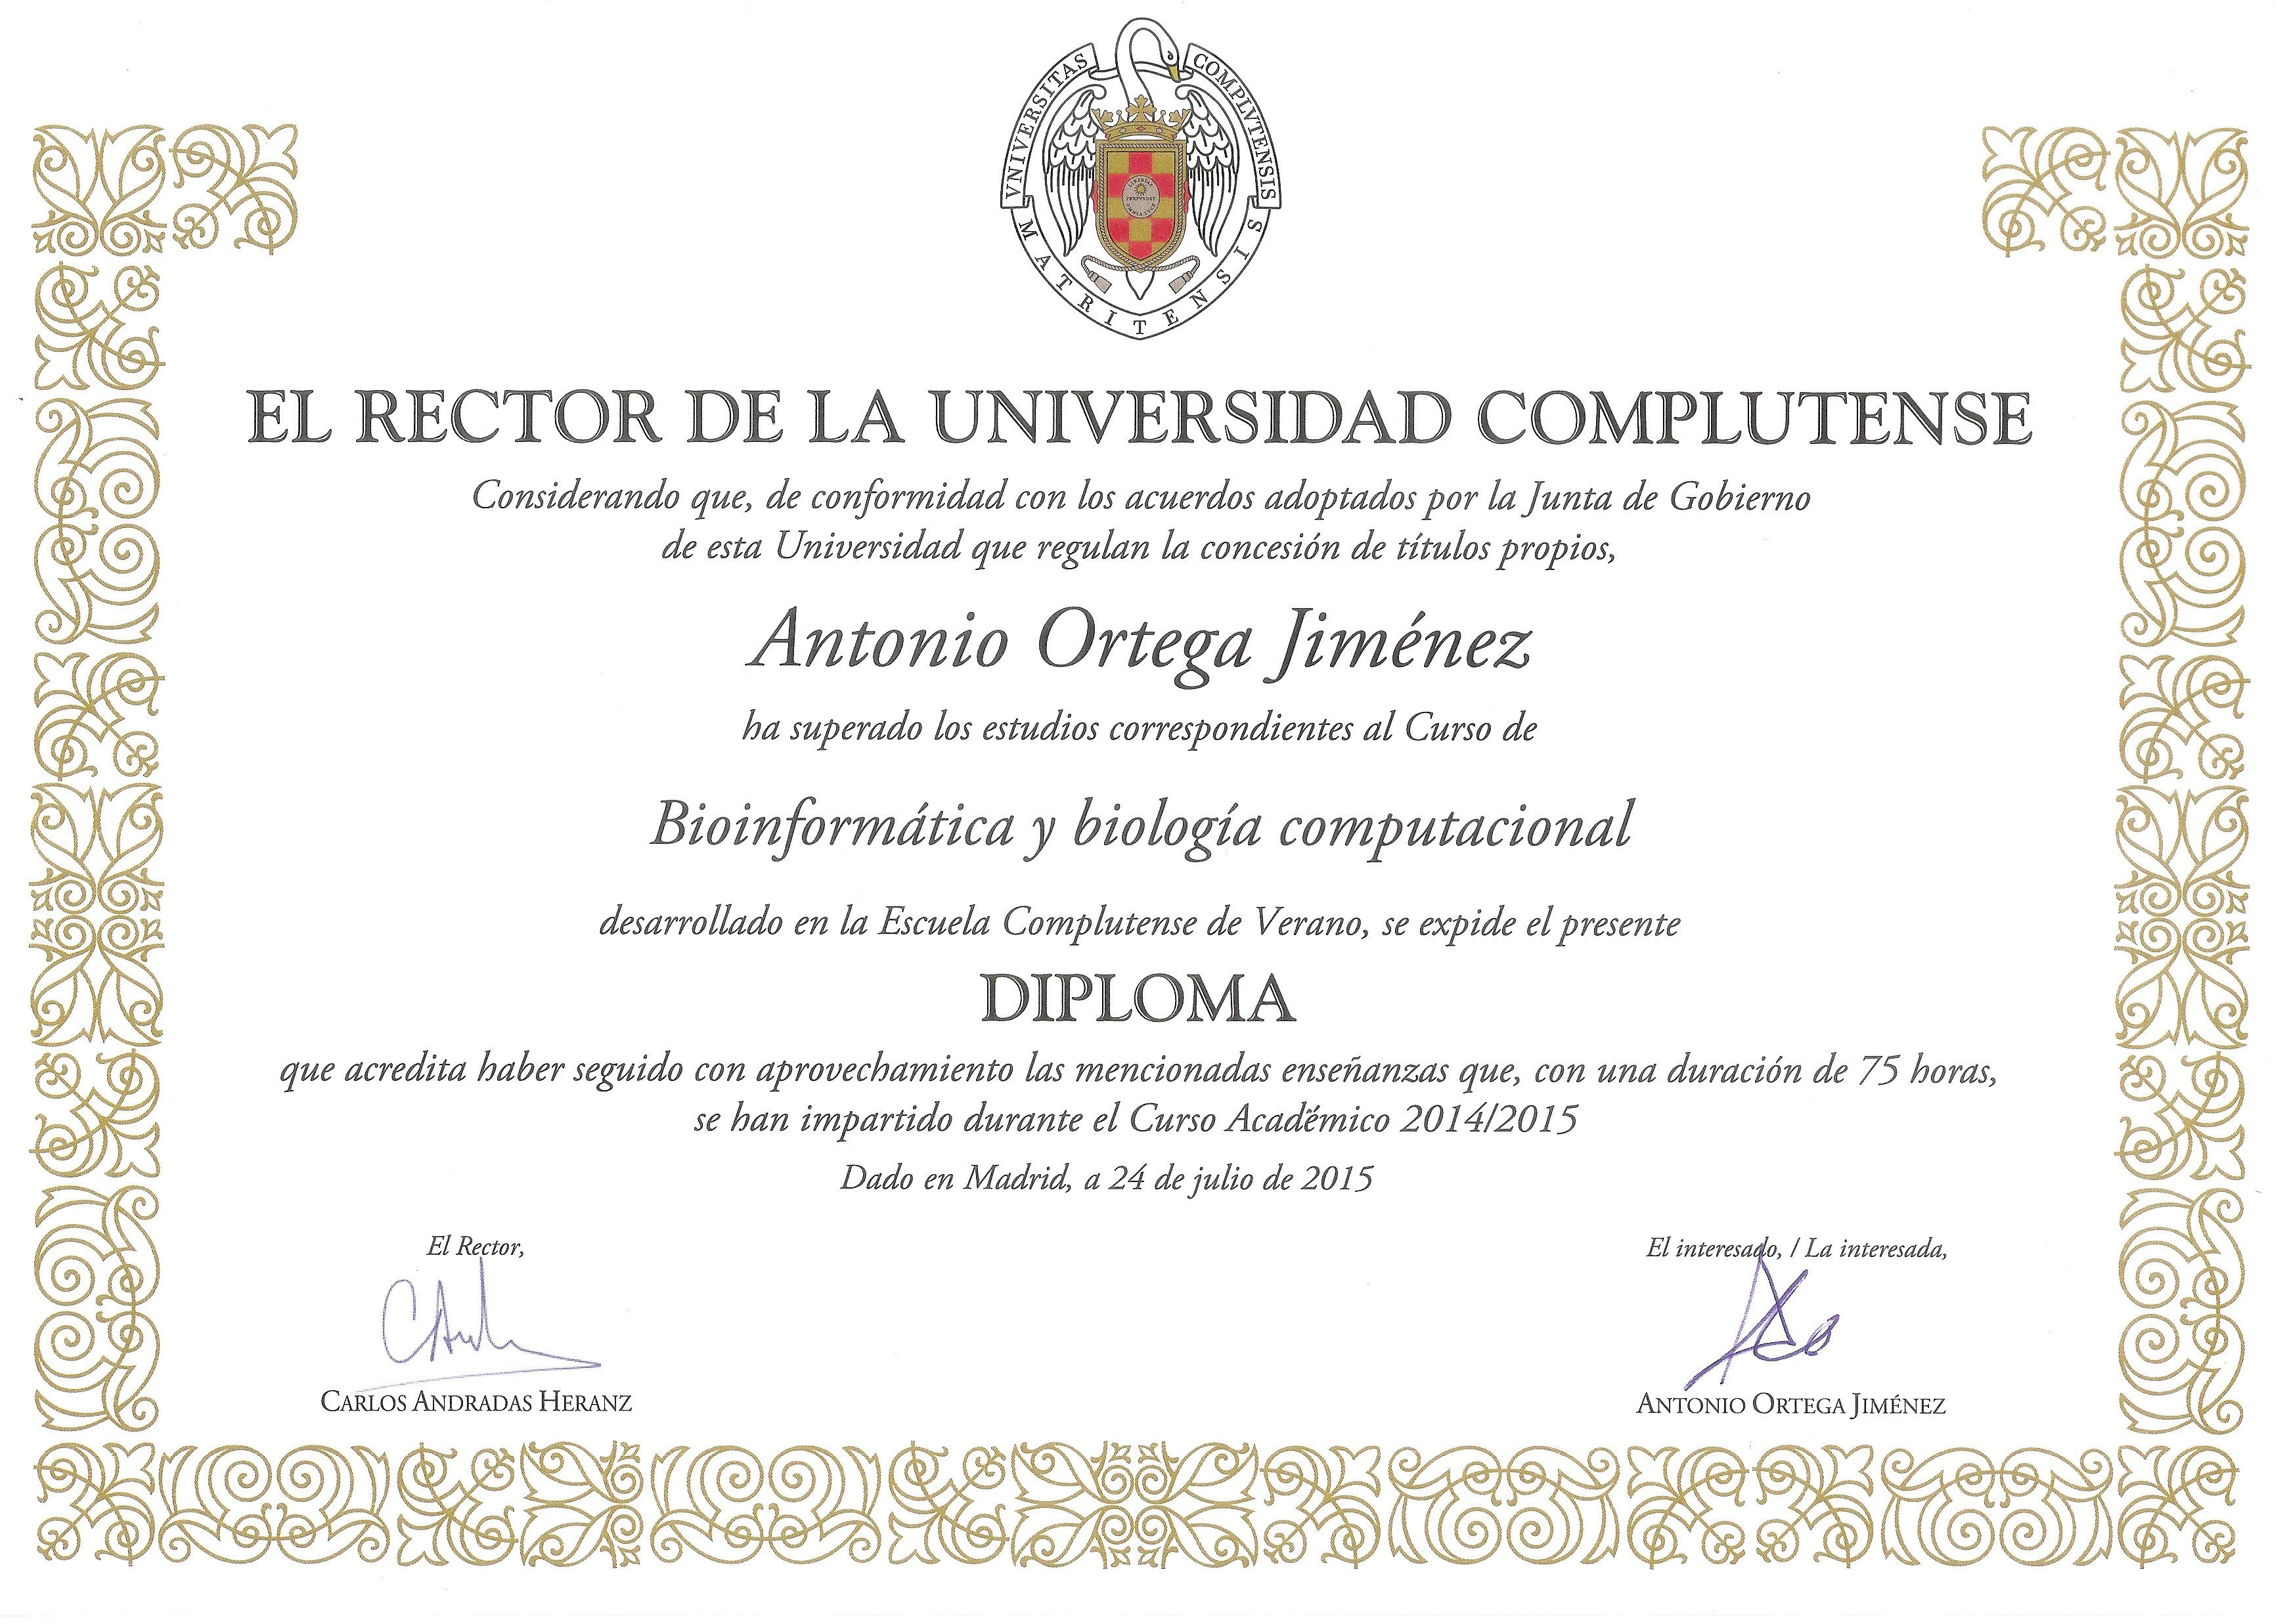
\includegraphics[scale=0.2]{./bioinformatica2.jpg}
\end{landscape}
\restoregeometry
\clearpage



%Expediente oficial en inglés
\hypertarget{exp-en}{}
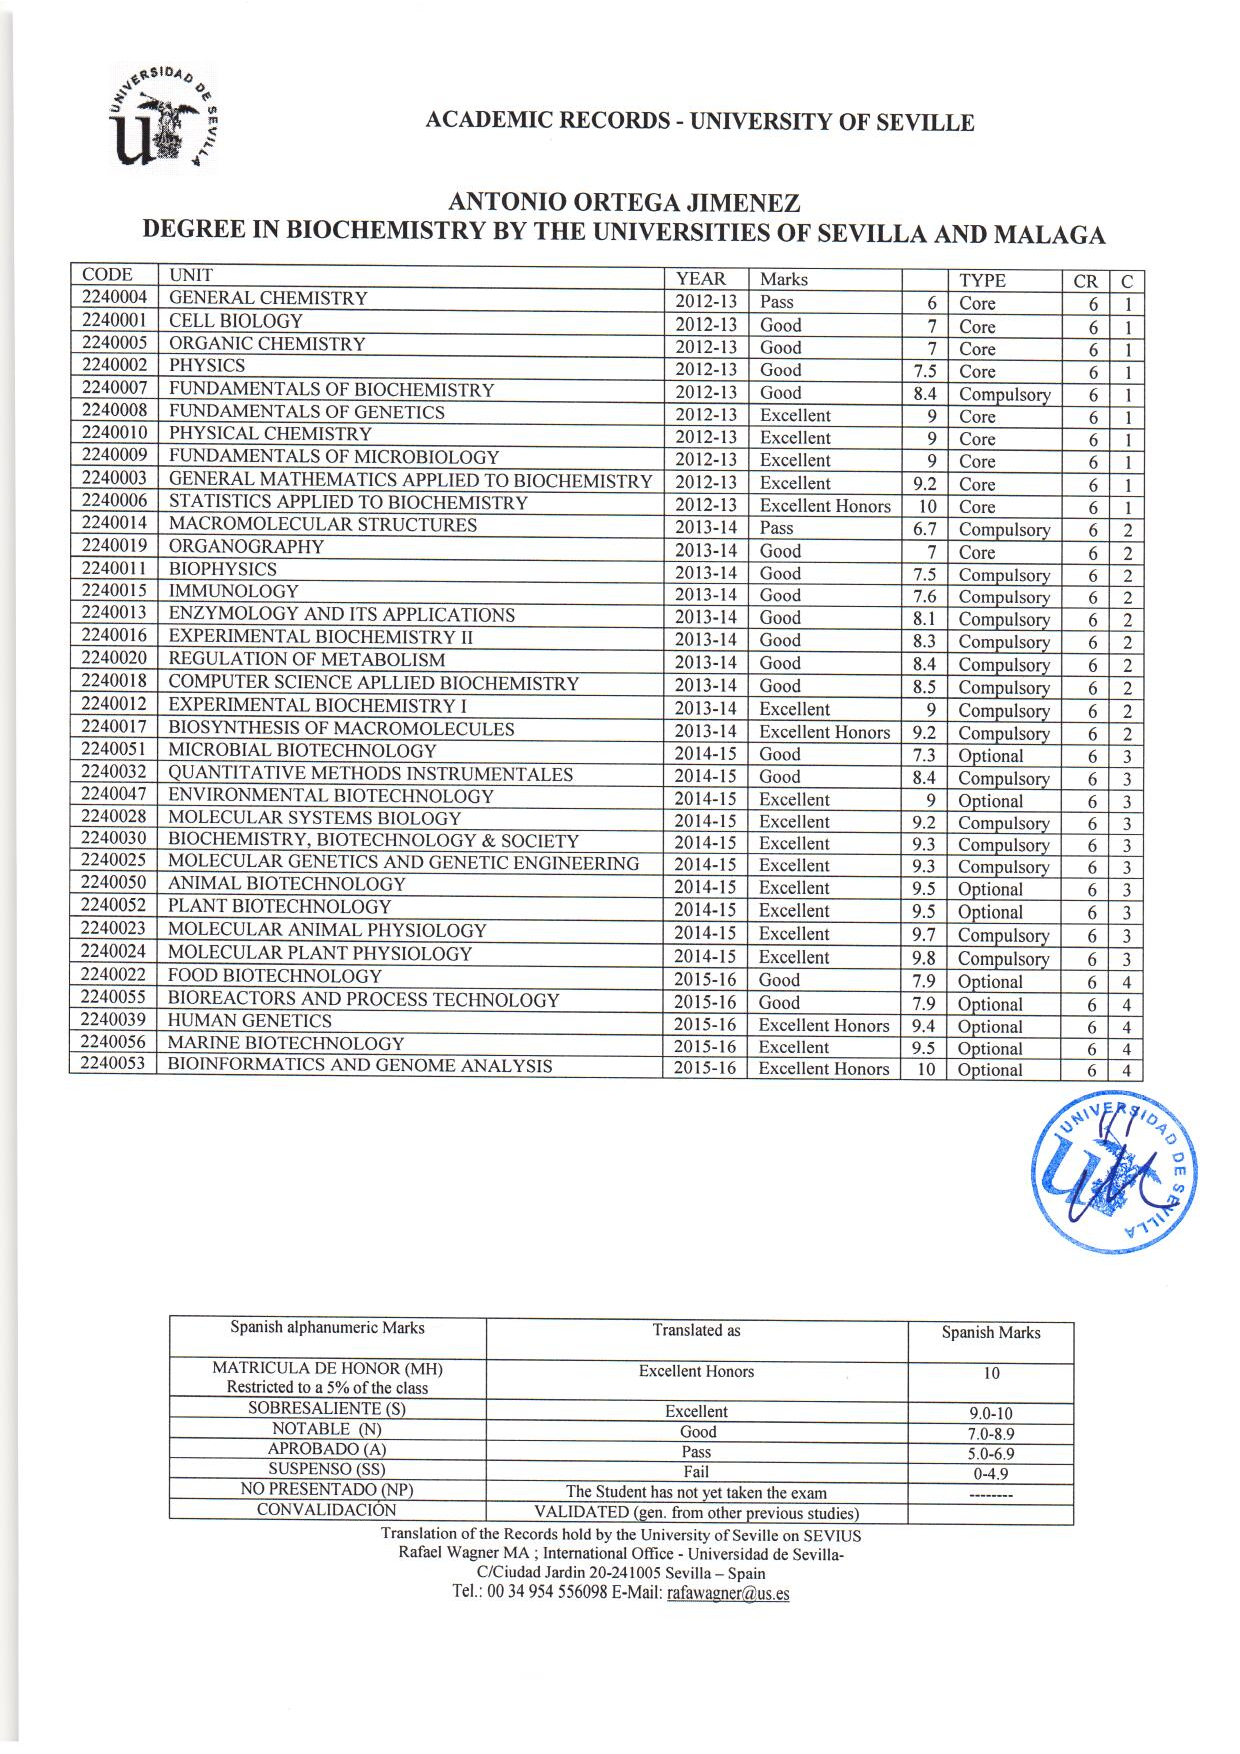
\includepdf[pages={1}]{Transcript-English.pdf}
\clearpage


\hypertarget{cae}{}
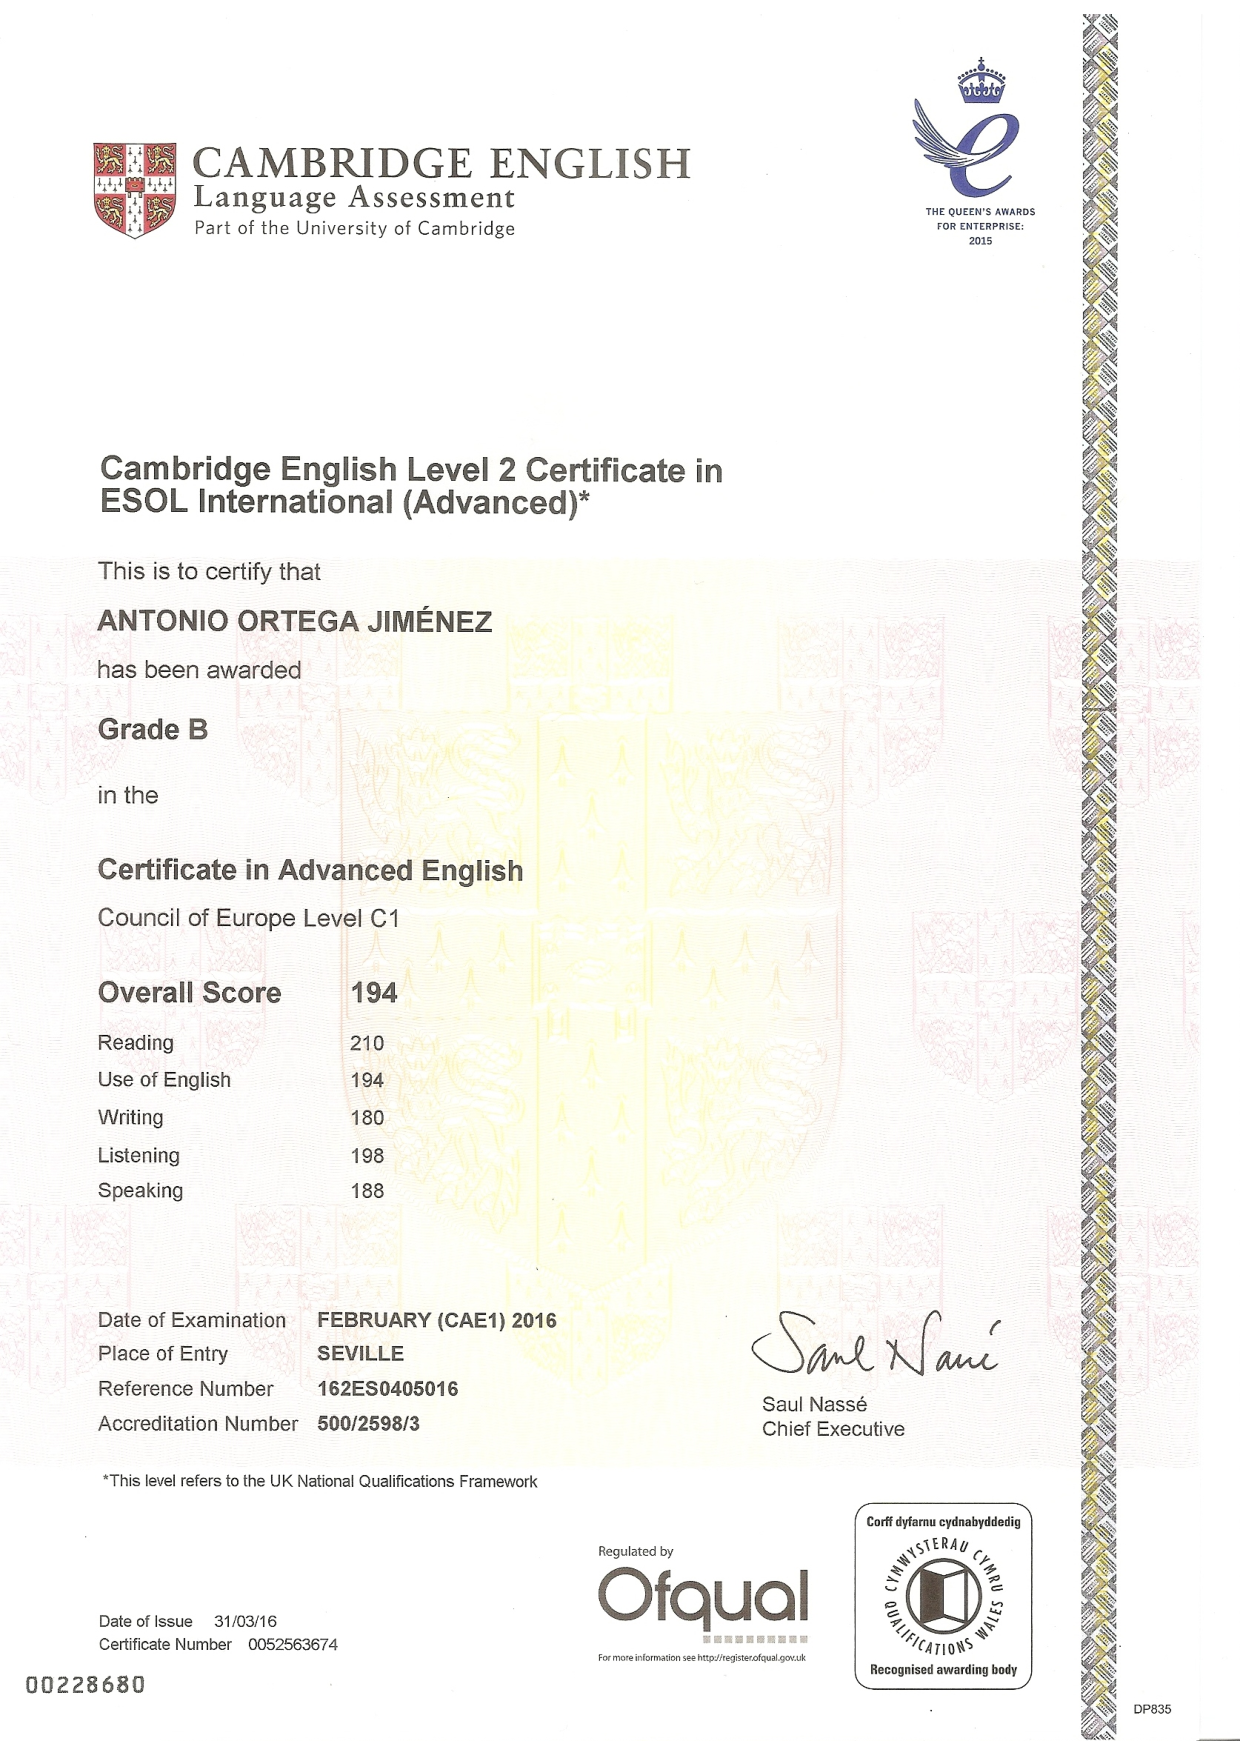
\includepdf{cae.pdf}
\clearpage



%Certificado DELF
%\thispagestyle{empty}
%\begin{landscape}
%\begin{figure}
%\hspace{-2.5 cm}
%\includegraphics[scale=0.3]{./delf.jpg}
%\end{figure}
%\end{landscape}
%\clearpage


\end{document}
